\documentclass{beamer}

\usepackage[utf8]{inputenc}
\usepackage{ngerman}
\usepackage{graphics}
\usepackage{multimedia}

\usetheme{Warsaw}
%\usecolortheme[named=orange]{structure}
%\useinnertheme{rectangles}

\setbeamercovered{transparent}

\beamertemplatenavigationsymbolsempty

\title{Tschernobyl}
\date{\today}
\institute{Friedrich Engels Gymnasium - Biologie}
\titlegraphic{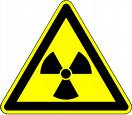
\includegraphics[width=3cm]{img/atomwarn.jpg}}
\author[T.Arnold \& L.Selke]{Theresa Arnold \and Laura Selke}


\setbeamertemplate{sections/subsections in toc}[rounded] 
\setbeamercolor{section number projected}{fg=blue!10!white,bg=black}
\setbeamercolor{section in toc}{fg=blue!40!black}
\setbeamercolor{subsection in toc}{fg=black}

\begin{document}
\begin{frame}
    \titlepage
\end{frame}

\section*{Inhaltsverzeichnis}
\begin{frame}{Inhaltsverzeichnis}
    \tableofcontents[pausesections]
\end{frame}

\section{Allgemeine Hintergründe}
\frame{\begin{block}{}\begin{center}\Huge{\textbf{Allgemeine Hintergründe}}\end{center}\end{block}}
\begin{frame}{}
    \begin{center}
        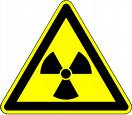
\includegraphics[width=7.5cm]{img/atomwarn.jpg}\\
    \end{center}
\end{frame}

\begin{frame}{}
    \begin{center}
        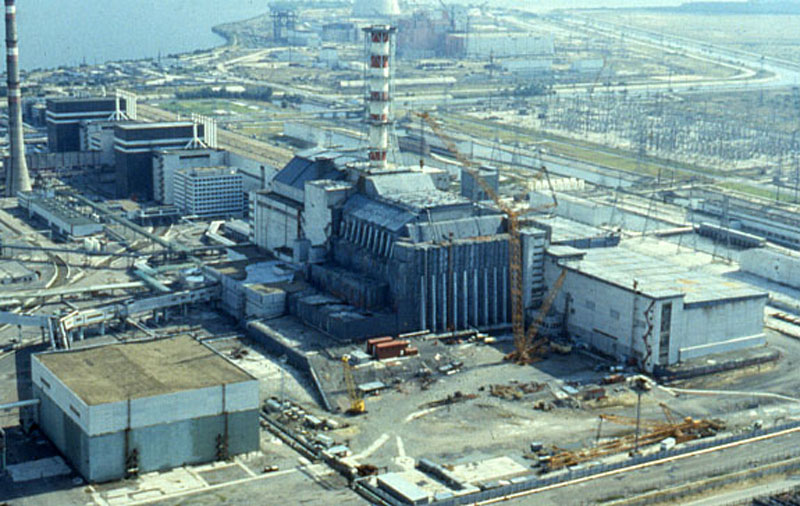
\includegraphics[width=7.5cm]{img/allgemein2.jpg}\\
        \begin{block}{}
            \center{Tschnernobyl vor dem Unglück}
        \end{block}
    \end{center}
\end{frame}

\begin{frame}{}
    \begin{center}
        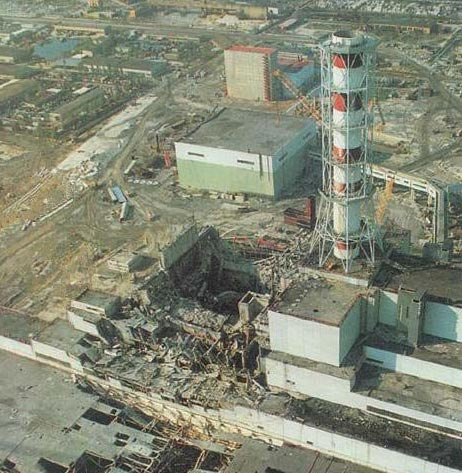
\includegraphics[height=6.0cm]{img/allgemein3}\\
        \begin{block}{}
            \center{Tschnernobyl nach dem Unglück}
        \end{block}
    \end{center}
\end{frame}

\begin{frame}{}
    \begin{center}
        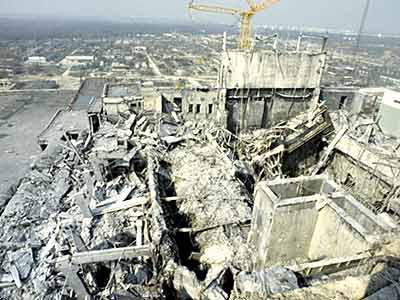
\includegraphics[width=7.5cm]{img/allgemein4}\\
        \begin{block}{}
            \center{Tschernobyl nach dem Unglück}
        \end{block}
    \end{center}
\end{frame}

\section{Kontaminierte Gebiete}
\frame{\begin{block}{}\begin{center}\Huge{\textbf{Kontaminierte Gebiete}}\end{center}\end{block}}
\begin{frame}{}
    \begin{center}
        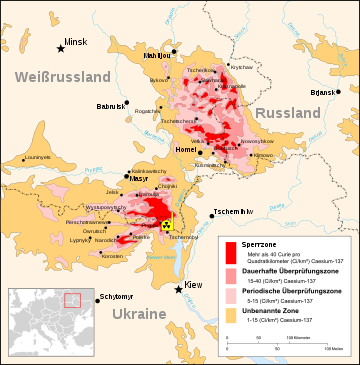
\includegraphics[height=6.0cm]{img/Kontaminierte_gebiete_1.jpg}\\
        \begin{block}{}
            \center{Ukraine, Weißrussland, Russland}
        \end{block}
    \end{center}
\end{frame}

\begin{frame}{}
    \begin{center}
        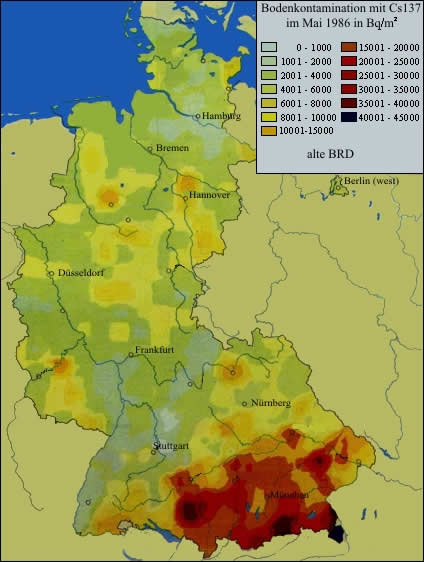
\includegraphics[height=6.0cm]{img/Kontaminierte_gebiete_2.jpg}\\
        \begin{block}{}
            \center{Auswirkungen auf Deutschland}
        \end{block}
    \end{center}
\end{frame}

\begin{frame}{}
    \begin{center}
        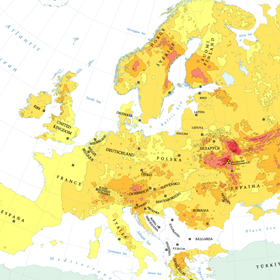
\includegraphics[height=6.0cm]{img/Kontaminierte_gebiete_3.jpg}\\
        \begin{block}{}
            \center{Auswirkungen auf Europa}
        \end{block}
    \end{center}
\end{frame}

\section{Gesundheitliche Folgen}
\frame{\begin{block}{}\begin{center}\Huge{\textbf{Gesundheitliche Folgen}}\end{center}\end{block}}

\begin{frame}
    \begin{columns}
        \column{.5\textwidth}
        \center{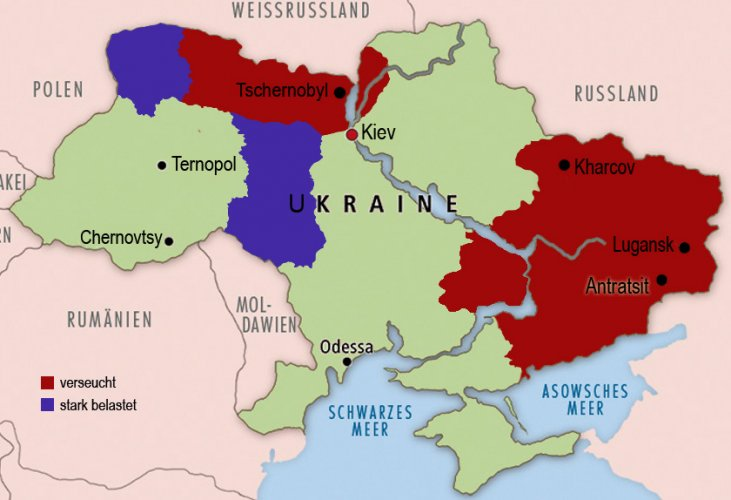
\includegraphics[width=5cm]{img/Bild_1a.jpg}}
        \column{.5\textwidth}
        \center{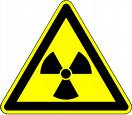
\includegraphics[width=5cm]{img/Bild_1b.jpg}}
    \end{columns}
    \begin{block}{}
        \center{Kontaminierte Gebiete}
    \end{block}
\end{frame}

\begin{frame}
    \begin{center}
        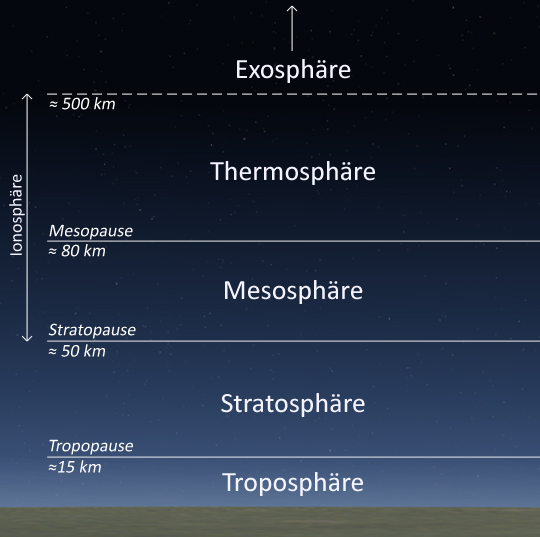
\includegraphics[height=6.0cm]{img/Bild_2.jpg}\\
        \begin{block}{}
            \center{Sphären}
        \end{block}
    \end{center}
\end{frame}

\begin{frame}
    \begin{columns}
        \column{.5\textwidth}
        \center{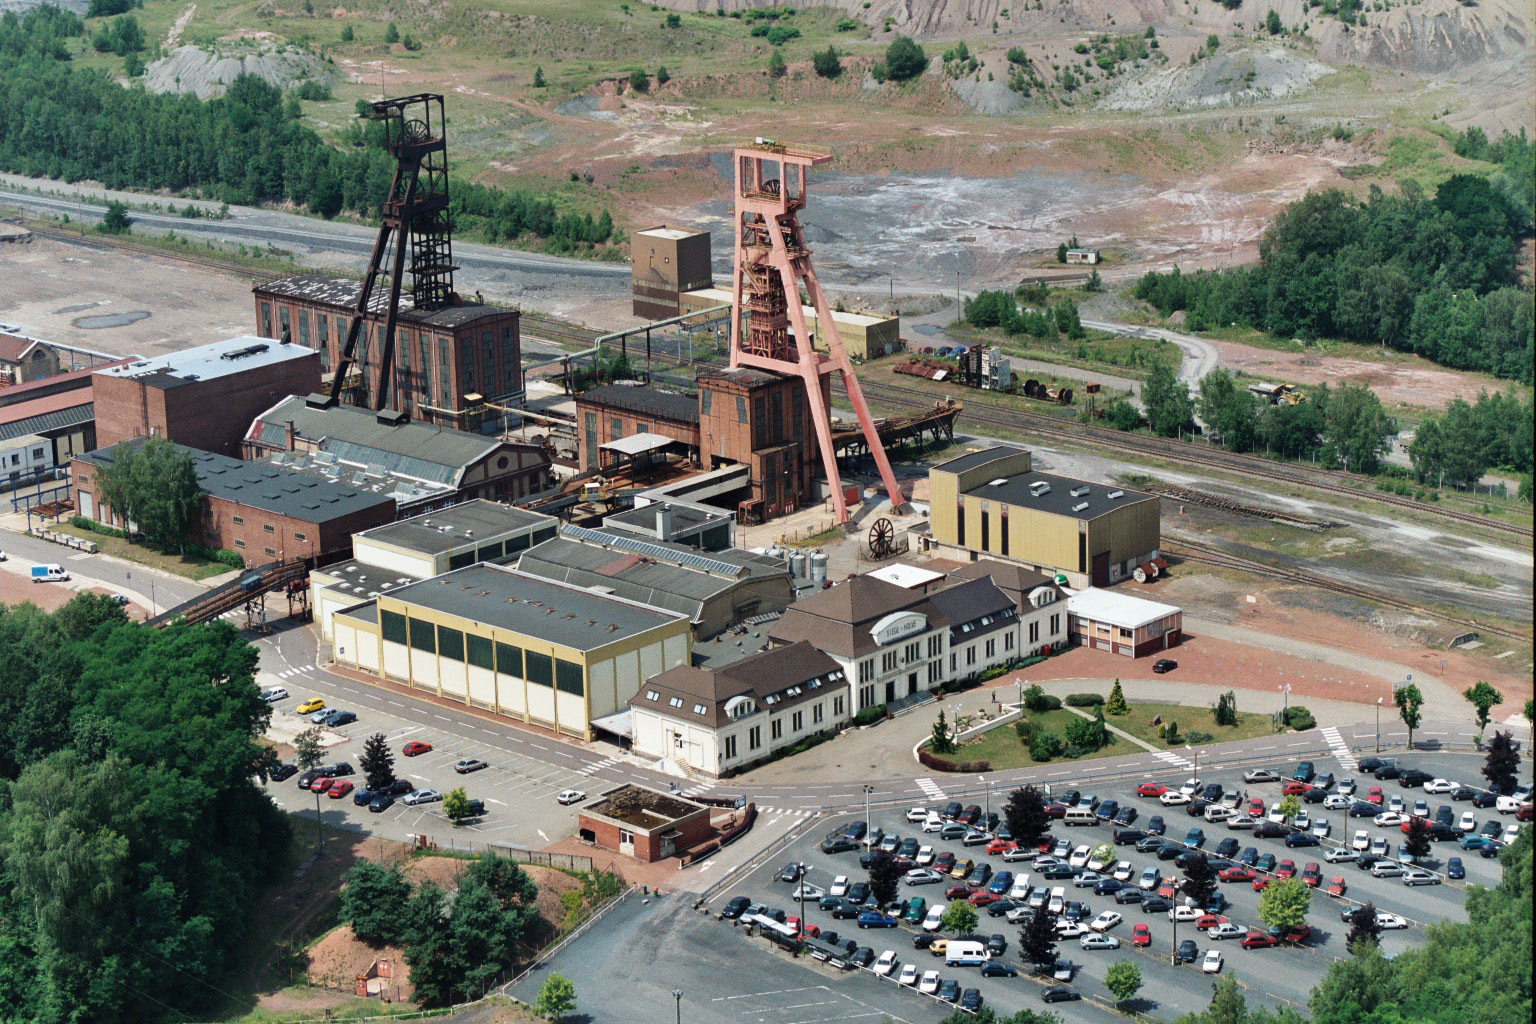
\includegraphics[width=5cm]{img/Bild_3a.jpg}}
        \column{.5\textwidth}
        \center{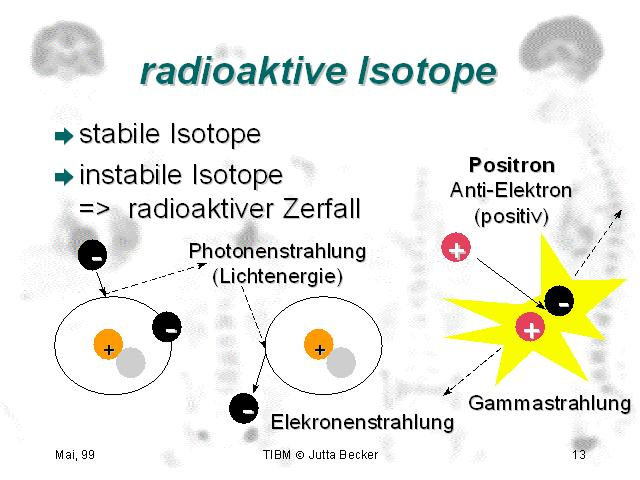
\includegraphics[width=5cm]{img/Bild_3b.jpg}}
    \end{columns}
    \begin{block}{}
        \center{Radioaktive Isotope}
    \end{block}
\end{frame}

\begin{frame}
    \begin{center}
        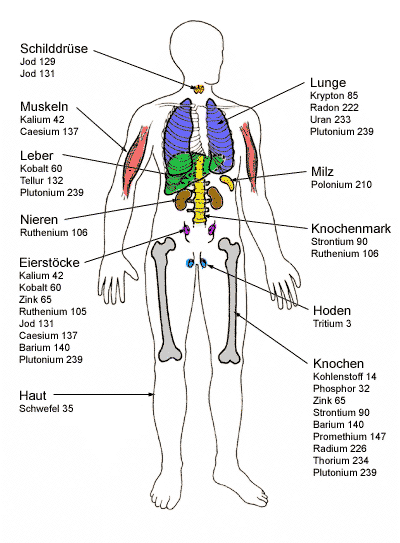
\includegraphics[height=6.0cm]{img/Bild_4b.png}\\
        \begin{block}{}
            \center{Betroffene Organe}
        \end{block}
    \end{center}
\end{frame}

\section{Genetische Veränderungen}
\frame{\begin{block}{}\begin{center}\Huge{\textbf{Genetische Veränderungen}}\end{center}\end{block}}

\begin{frame}
    \begin{center}
        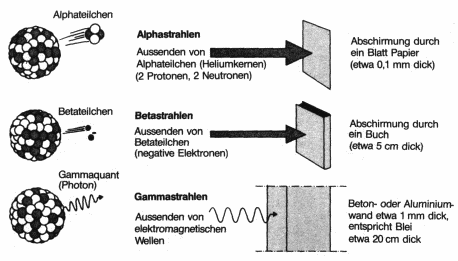
\includegraphics[width=7.5cm]{img/Bild_5.png}\\
        \begin{block}{}
            \center{Radioaktive Strahlungen}
        \end{block}
    \end{center}
\end{frame}

\begin{frame}
    \begin{columns}
        \column{.5\textwidth}
        \center{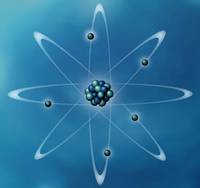
\includegraphics[width=5cm]{img/Bild_6_geloeste_elektronen.jpg}}
        \column{.5\textwidth}
        \center{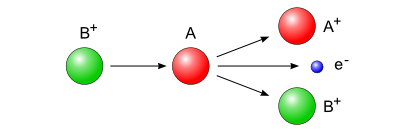
\includegraphics[width=5cm]{img/Bild_6a.png}}
    \end{columns}
    \begin{block}{}
        \center{Gelöste Elektronen}
    \end{block}
\end{frame}

\begin{frame}{}
    \begin{center}
        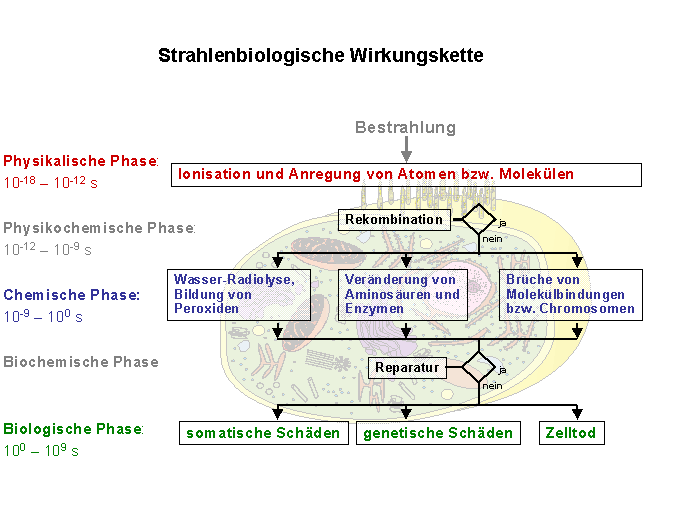
\includegraphics[width=7.5cm]{img/Bild_7.png}\\
        \begin{block}{}
            \center{Bestrahlung}
        \end{block}
    \end{center}
\end{frame}

\begin{frame}{}
    \begin{columns}
        \column{.5\textwidth}
        \center{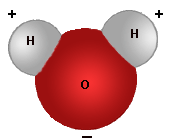
\includegraphics[width=5cm]{img/Bild_8a.png}}
        \column{.5\textwidth}
        \center{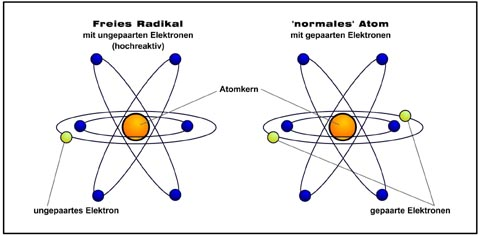
\includegraphics[width=5cm]{img/Bild_8b.jpg}}
    \end{columns}
\end{frame}

\begin{frame}{}
    \begin{center}
        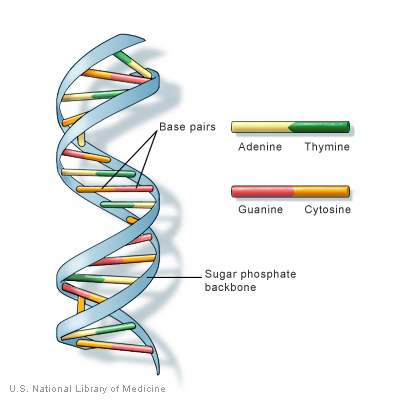
\includegraphics[height=6.0cm]{img/Bild_9_langfristige_Folgen.jpg}\\
        \begin{block}{}
            \center{Langfristige Folgen}
        \end{block}
    \end{center}
\end{frame}

\begin{frame}
    \begin{center}
        \begin{block}{}
            \center{\movie[poster, autostart, externalviewer, loop]{Schädigung der Basen}{schaedigungDerBasen.gif}}
        \end{block}
        \begin{block}{}
            \center{\movie[poster, autostart, externalviewer, loop]{Einzelstrangbruch}{Einzelstrangbruch.gif}}
        \end{block}
        \begin{block}{}
            \center{\movie[poster, autostart, externalviewer, loop]{Doppelstrangbruch}{Doppelstrangbruch.gif}}
        \end{block}
    \end{center}
\end{frame}

\begin{frame}{}
    \begin{center}
        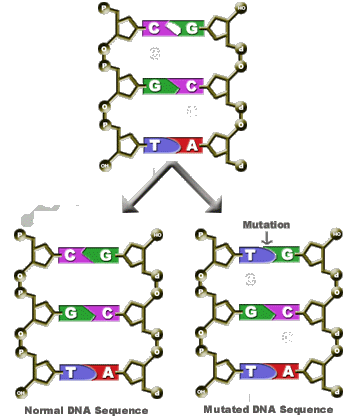
\includegraphics[height=6.0cm]{img/Bild_11_Quervernetzung.png}\\
        \begin{block}{}
            \center{Quervernetzung}
        \end{block}
    \end{center}
\end{frame}

\section{Tschernobyl Heute}
\frame{\begin{block}{}\begin{center}\Huge{\textbf{Tschnerobyl Heute}}\end{center}\end{block}}

\begin{frame}[plain]{}
    \begin{center}
        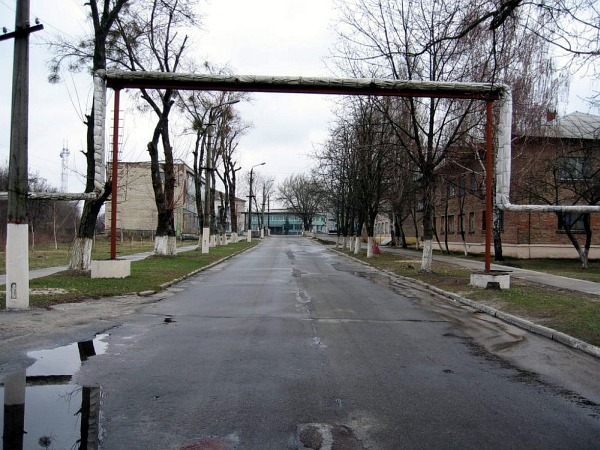
\includegraphics[width=11cm]{img/heute1.jpg}\\
    \end{center}
\end{frame}

\begin{frame}[plain]{}
    \begin{center}
        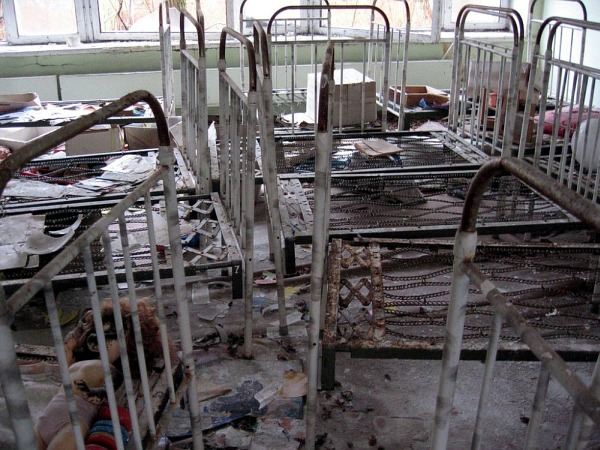
\includegraphics[width=11cm]{img/Heute_2.jpg}\\
    \end{center}
\end{frame}

\begin{frame}[plain]{}
    \begin{center}
        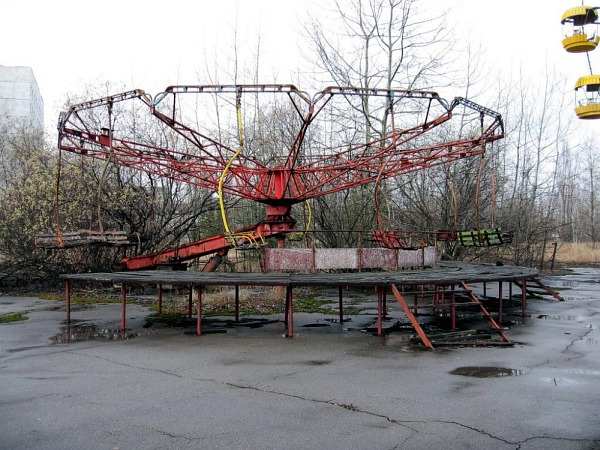
\includegraphics[width=11cm]{img/Heute_3.jpg}\\
    \end{center}
\end{frame}

\begin{frame}[plain]{}
    \begin{center}
        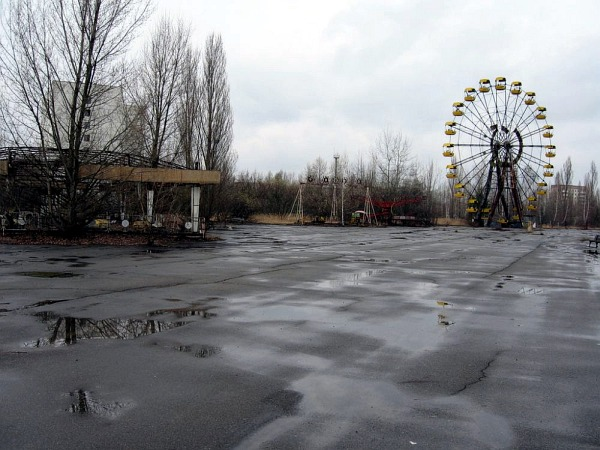
\includegraphics[width=11cm]{img/Heute_4.jpg}\\
    \end{center}
\end{frame}

\begin{frame}
    \begin{block}{}
        \begin{center}
            \textbf{In Deutschland stehen immer noch 17 Atomkraftwerke\\[1em]
            Allein im Jahr 2004 gab es 113 meldepflichtige Störfälle.}
        \end{center}
    \end{block}
\end{frame}

\section*{Quellen}
\frame{\begin{block}{}\begin{center}\Huge{\textbf{Quellen}}\end{center}\end{block}}

\begin{frame}
    \begin{block}{Internet}
        \begin{tiny}
http://www.noezsv.at/wissenhilft/radioaktivitaet/wirkungaufmensch.htm\\
http://www.krebsinformationsdienst.de/themen/risiken/radioaktivitaet-und-roentgenstrahlen.php\\
http://www.reyl.de/tschernobyl/\\
http://www.greenpeace-berlin.de/tschernobyl/\\
http://www.greenpeace.at/tschernobyl.html\\
http://www.pausenhof.de/referat/physik/tschernobyl/12426\\
        \end{tiny}
    \end{block}
    \begin{block}{Bücher}
        \begin{tiny}
Reimar Paul - Basiswissen Atomkraftwerke\\
Reimar Paul - Der gefährliche Traum Atomkraft\\
Bayrisches Staatsministerium für Umwelt, Gesundheit und Verbraucherschutz - Radioaktivität, Röntgenstrahlen und Gesundheit\\
Duden- Genetikn\\
        \end{tiny}
    \end{block}
    \pause
\end{frame}

\end{document}
